\documentclass[11pt,a4paper]{article}

% Packages
\usepackage[utf8]{inputenc}
\usepackage[T1]{fontenc}
\usepackage{lmodern}
\usepackage[margin=1in]{geometry}
\usepackage{graphicx}
\usepackage{tikz}
\usetikzlibrary{shapes.geometric, arrows, positioning, fit, backgrounds, calc}
\usepackage{listings}
\usepackage{xcolor}
\usepackage{hyperref}
\usepackage{booktabs}
\usepackage{amsmath}
\usepackage{amssymb}
\usepackage{float}
\usepackage{enumitem}
\usepackage{fancyhdr}
\usepackage{tocloft}

% Colors
\definecolor{codegreen}{rgb}{0,0.6,0}
\definecolor{codegray}{rgb}{0.5,0.5,0.5}
\definecolor{codepurple}{rgb}{0.58,0,0.82}
\definecolor{backcolour}{rgb}{0.95,0.95,0.92}
\definecolor{classcolor}{RGB}{173,216,230}
\definecolor{modulecolor}{RGB}{144,238,144}
\definecolor{interfacecolor}{RGB}{255,218,185}

% Code listing style
\lstdefinestyle{pythonstyle}{
    backgroundcolor=\color{backcolour},
    commentstyle=\color{codegreen},
    keywordstyle=\color{magenta},
    numberstyle=\tiny\color{codegray},
    stringstyle=\color{codepurple},
    basicstyle=\ttfamily\footnotesize,
    breakatwhitespace=false,
    breaklines=true,
    captionpos=b,
    keepspaces=true,
    numbers=left,
    numbersep=5pt,
    showspaces=false,
    showstringspaces=false,
    showtabs=false,
    tabsize=2,
    language=Python
}
\lstset{style=pythonstyle}

% Header/Footer
\pagestyle{fancy}
\fancyhf{}
\rhead{AutoML QSAR Documentation}
\lhead{\leftmark}
\rfoot{Page \thepage}

% Title
\title{
    \vspace{-2cm}
    \textbf{AutoML QSAR Pipeline}\\
    \large Automated Machine Learning for Quantitative Structure-Activity Relationship Modeling\\
    \vspace{0.5cm}
    \large Technical Documentation \& Architecture
}
\author{QSAR Development Team}
\date{\today}

\begin{document}

\maketitle
\tableofcontents
\newpage

% ============================================================================
\section{Introduction}
% ============================================================================

\subsection{Overview}

The \textbf{AutoML QSAR Pipeline} is a comprehensive automated machine learning framework designed for predicting biological activity of molecules based on their chemical structure. This system automates the entire workflow from data curation to model deployment, making QSAR modeling accessible and reproducible.

\subsection{Key Features}

\begin{itemize}[leftmargin=*]
    \item \textbf{Automated Data Curation}: SMILES validation, duplicate handling, task type inference
    \item \textbf{Multi-Task Support}: Regression, classification, and mixed task handling
    \item \textbf{Multiple Featurization Methods}: RDKit descriptors, ECFP fingerprints, MACCS keys
    \item \textbf{Ensemble Learning}: Combines multiple models for robust predictions
    \item \textbf{Hyperparameter Optimization}: Bayesian optimization with Optuna
    \item \textbf{Uncertainty Quantification}: Provides confidence estimates for predictions
    \item \textbf{Model Persistence}: Save and load trained models
\end{itemize}

\subsection{Scientific Background}

QSAR (Quantitative Structure-Activity Relationship) models establish mathematical relationships between molecular structure and biological activity. The fundamental equation is:

\begin{equation}
    \text{Activity} = f(\text{Molecular Descriptors})
\end{equation}

For IC50 (half-maximal inhibitory concentration) prediction, we use the pIC50 transformation:

\begin{equation}
    \text{pIC50} = -\log_{10}(\text{IC50}_M) = 9 - \log_{10}(\text{IC50}_{nM})
\end{equation}

This logarithmic transformation provides:
\begin{itemize}
    \item Normal distribution of target values
    \item Equal weighting across activity ranges
    \item Interpretable units (higher pIC50 = more potent)
\end{itemize}

% ============================================================================
\section{System Architecture}
% ============================================================================

\subsection{High-Level Architecture}

\begin{figure}[H]
\centering
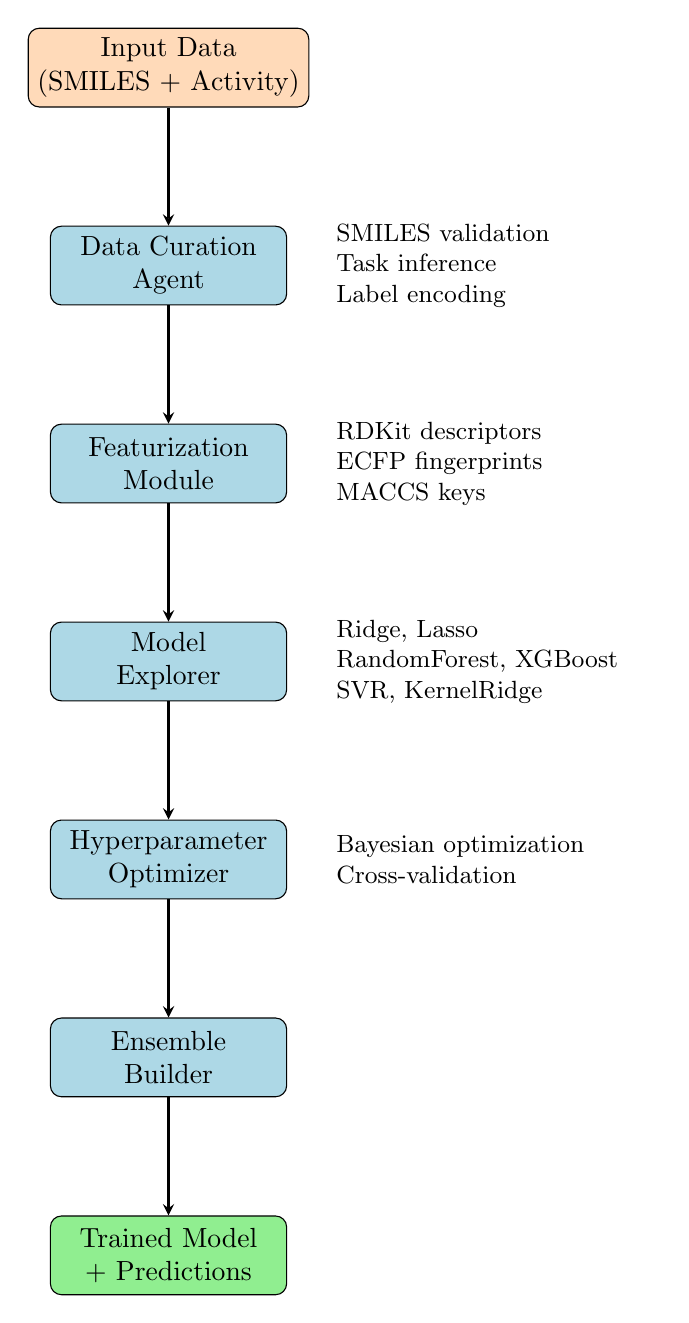
\begin{tikzpicture}[
    node distance=1.5cm,
    box/.style={rectangle, draw, rounded corners, minimum width=3cm, minimum height=1cm, align=center, fill=classcolor},
    arrow/.style={->, >=stealth, thick}
]
    % Input
    \node[box, fill=interfacecolor] (input) {Input Data\\(SMILES + Activity)};
    
    % Processing pipeline
    \node[box, below=of input] (curation) {Data Curation\\Agent};
    \node[box, below=of curation] (feature) {Featurization\\Module};
    \node[box, below=of feature] (model) {Model\\Explorer};
    \node[box, below=of model] (optimize) {Hyperparameter\\Optimizer};
    \node[box, below=of optimize] (ensemble) {Ensemble\\Builder};
    
    % Output
    \node[box, fill=modulecolor, below=of ensemble] (output) {Trained Model\\+ Predictions};
    
    % Arrows
    \draw[arrow] (input) -- (curation);
    \draw[arrow] (curation) -- (feature);
    \draw[arrow] (feature) -- (model);
    \draw[arrow] (model) -- (optimize);
    \draw[arrow] (optimize) -- (ensemble);
    \draw[arrow] (ensemble) -- (output);
    
    % Side annotations
    \node[right=0.5cm of curation, text width=4cm, font=\small] {SMILES validation\\Task inference\\Label encoding};
    \node[right=0.5cm of feature, text width=4cm, font=\small] {RDKit descriptors\\ECFP fingerprints\\MACCS keys};
    \node[right=0.5cm of model, text width=4cm, font=\small] {Ridge, Lasso\\RandomForest, XGBoost\\SVR, KernelRidge};
    \node[right=0.5cm of optimize, text width=4cm, font=\small] {Bayesian optimization\\Cross-validation};
    
\end{tikzpicture}
\caption{High-Level Pipeline Architecture}
\end{figure}

\subsection{Package Structure}

\begin{figure}[H]
\centering
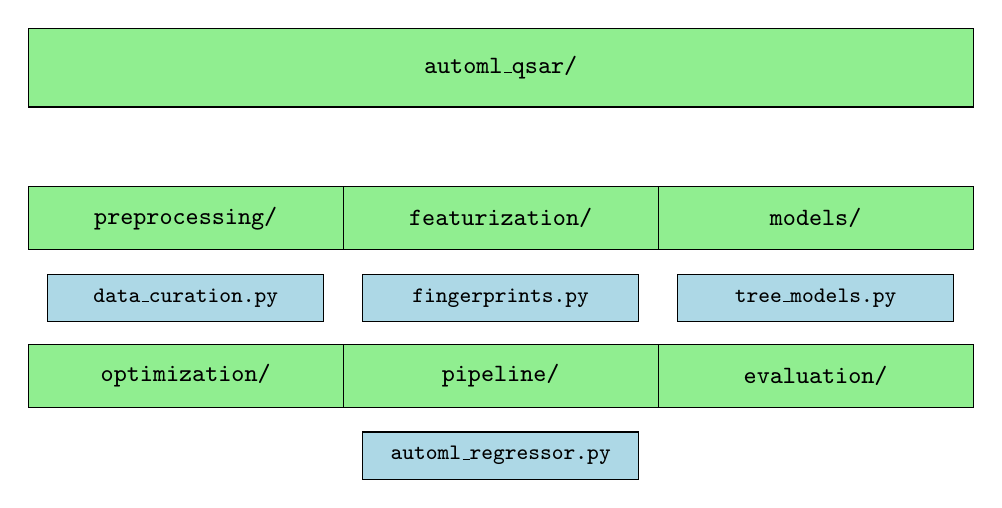
\begin{tikzpicture}[
    node distance=0.8cm,
    package/.style={rectangle, draw, minimum width=4cm, minimum height=0.8cm, fill=modulecolor, font=\ttfamily\small},
    module/.style={rectangle, draw, minimum width=3.5cm, minimum height=0.6cm, fill=classcolor, font=\ttfamily\footnotesize},
    arrow/.style={->, >=stealth}
]
    % Main package
    \node[package, minimum width=12cm, minimum height=1cm] (main) {automl\_qsar/};
    
    % Subpackages - Row 1
    \node[package, below=1cm of main, xshift=-4cm] (preprocess) {preprocessing/};
    \node[package, below=1cm of main] (feature) {featurization/};
    \node[package, below=1cm of main, xshift=4cm] (models) {models/};
    
    % Subpackages - Row 2
    \node[package, below=3cm of main, xshift=-4cm] (optimize) {optimization/};
    \node[package, below=3cm of main] (pipeline) {pipeline/};
    \node[package, below=3cm of main, xshift=4cm] (eval) {evaluation/};
    
    % Modules under preprocessing
    \node[module, below=0.3cm of preprocess] (dc) {data\_curation.py};
    
    % Modules under featurization
    \node[module, below=0.3cm of feature] (fp) {fingerprints.py};
    
    % Modules under models
    \node[module, below=0.3cm of models] (tree) {tree\_models.py};
    
    % Modules under pipeline
    \node[module, below=0.3cm of pipeline] (automl) {automl\_regressor.py};
    
\end{tikzpicture}
\caption{Package Structure}
\end{figure}

% ============================================================================
\section{UML Class Diagrams}
% ============================================================================

\subsection{Data Curation Module}

\begin{figure}[H]
\centering
\begin{tikzpicture}[
    class/.style={rectangle, draw, minimum width=6cm, font=\small},
    classname/.style={rectangle, draw, fill=classcolor, minimum width=6cm, font=\bfseries\small},
    enum/.style={rectangle, draw, fill=interfacecolor, minimum width=4cm, font=\small},
    enumname/.style={rectangle, draw, fill=interfacecolor!70, minimum width=4cm, font=\bfseries\small},
    arrow/.style={->, >=open triangle 60, thick},
    composition/.style={-*, thick},
    node distance=0.1cm
]

    % TaskType Enum
    \node[enumname] (taskname) {\guillemotleft enumeration\guillemotright\\TaskType};
    \node[enum, below=0cm of taskname] (taskenum) {
        \begin{tabular}{l}
        REGRESSION\_SINGLE\\
        REGRESSION\_MULTI\\
        CLASSIFICATION\_BINARY\\
        CLASSIFICATION\_MULTICLASS\\
        CLASSIFICATION\_MULTILABEL\\
        MIXED\\
        UNKNOWN
        \end{tabular}
    };
    
    % TargetConfig dataclass
    \node[classname, right=2cm of taskname] (targetname) {\guillemotleft dataclass\guillemotright\\TargetConfig};
    \node[class, below=0cm of targetname] (targetattr) {
        \begin{tabular}{l}
        + name: str\\
        + task\_type: TaskType\\
        + unit: str = "nM"\\
        + apply\_log: bool = False\\
        + transform: str = "none"\\
        + label\_encoder: Any\\
        + classes: List[str]\\
        + statistics: Dict
        \end{tabular}
    };
    
    % QSARDataCurationAgent
    \node[classname, below=2cm of taskenum, xshift=3cm] (agentname) {QSARDataCurationAgent};
    \node[class, below=0cm of agentname] (agentattr) {
        \begin{tabular}{l}
        \textbf{Attributes:}\\
        - raw\_df: DataFrame\\
        - smiles\_col: str\\
        - target\_cols: List[str]\\
        - target\_configs: Dict[str, TargetConfig]\\
        - overall\_task: TaskType\\
        - cleaned\_df: DataFrame\\
        \hline
        \textbf{Methods:}\\
        + run() $\rightarrow$ DataFrame\\
        + get\_statistics() $\rightarrow$ Dict\\
        + get\_target\_configs() $\rightarrow$ Dict\\
        + get\_label\_encoder(col) $\rightarrow$ LabelEncoder\\
        - \_validate\_smiles()\\
        - \_infer\_task\_type(series) $\rightarrow$ TaskType\\
        - \_apply\_transformations()\\
        - \_encode\_labels()
        \end{tabular}
    };
    
    % Relationships
    \draw[arrow] (agentattr.north) -- ++(0,0.5) -| (taskenum.south);
    \draw[composition] (agentattr.north) -- ++(0,0.5) -| (targetattr.south);
    
\end{tikzpicture}
\caption{Data Curation Module Class Diagram}
\end{figure}

\subsection{Featurization Module}

\begin{figure}[H]
\centering
\begin{tikzpicture}[
    class/.style={rectangle, draw, minimum width=5cm, font=\small},
    classname/.style={rectangle, draw, fill=classcolor, minimum width=5cm, font=\bfseries\small},
    abstract/.style={rectangle, draw, fill=interfacecolor, minimum width=5cm, font=\small},
    abstractname/.style={rectangle, draw, fill=interfacecolor!70, minimum width=5cm, font=\bfseries\itshape\small},
    arrow/.style={->, >=open triangle 60, thick},
    node distance=0.1cm
]

    % BaseFeaturizer (Abstract)
    \node[abstractname] (basename) {\guillemotleft abstract\guillemotright\\BaseFeaturizer};
    \node[abstract, below=0cm of basename] (baseattr) {
        \begin{tabular}{l}
        + name: str\\
        + feature\_names: List[str]\\
        \hline
        + featurize(molecules) $\rightarrow$ ndarray\\
        \# \_smiles\_to\_mol(smiles) $\rightarrow$ Mol\\
        \# \_prepare\_molecules(mols) $\rightarrow$ List
        \end{tabular}
    };
    
    % Concrete implementations
    \node[classname, below=1.5cm of baseattr, xshift=-4cm] (rdkitname) {RDKitDescriptors};
    \node[class, below=0cm of rdkitname] (rdkitattr) {
        \begin{tabular}{l}
        + descriptor\_names: List\\
        \hline
        + featurize(smiles)\\
        $\rightarrow$ ndarray (n, 200+)
        \end{tabular}
    };
    
    \node[classname, below=1.5cm of baseattr] (ecfpname) {ECFPFingerprints};
    \node[class, below=0cm of ecfpname] (ecfpattr) {
        \begin{tabular}{l}
        + radius: int = 2\\
        + n\_bits: int = 1024\\
        \hline
        + featurize(smiles)\\
        $\rightarrow$ ndarray (n, 1024)
        \end{tabular}
    };
    
    \node[classname, below=1.5cm of baseattr, xshift=4cm] (maccsname) {MACCSFingerprints};
    \node[class, below=0cm of maccsname] (maccsattr) {
        \begin{tabular}{l}
        \hline
        + featurize(smiles)\\
        $\rightarrow$ ndarray (n, 167)
        \end{tabular}
    };
    
    % Inheritance arrows
    \draw[arrow] (rdkitname.north) -- ++(0,0.5) -| (baseattr.south);
    \draw[arrow] (ecfpname.north) -- (baseattr.south);
    \draw[arrow] (maccsname.north) -- ++(0,0.5) -| (baseattr.south);
    
\end{tikzpicture}
\caption{Featurization Module Class Diagram}
\end{figure}

\subsection{AutoML Pipeline}

\begin{figure}[H]
\centering
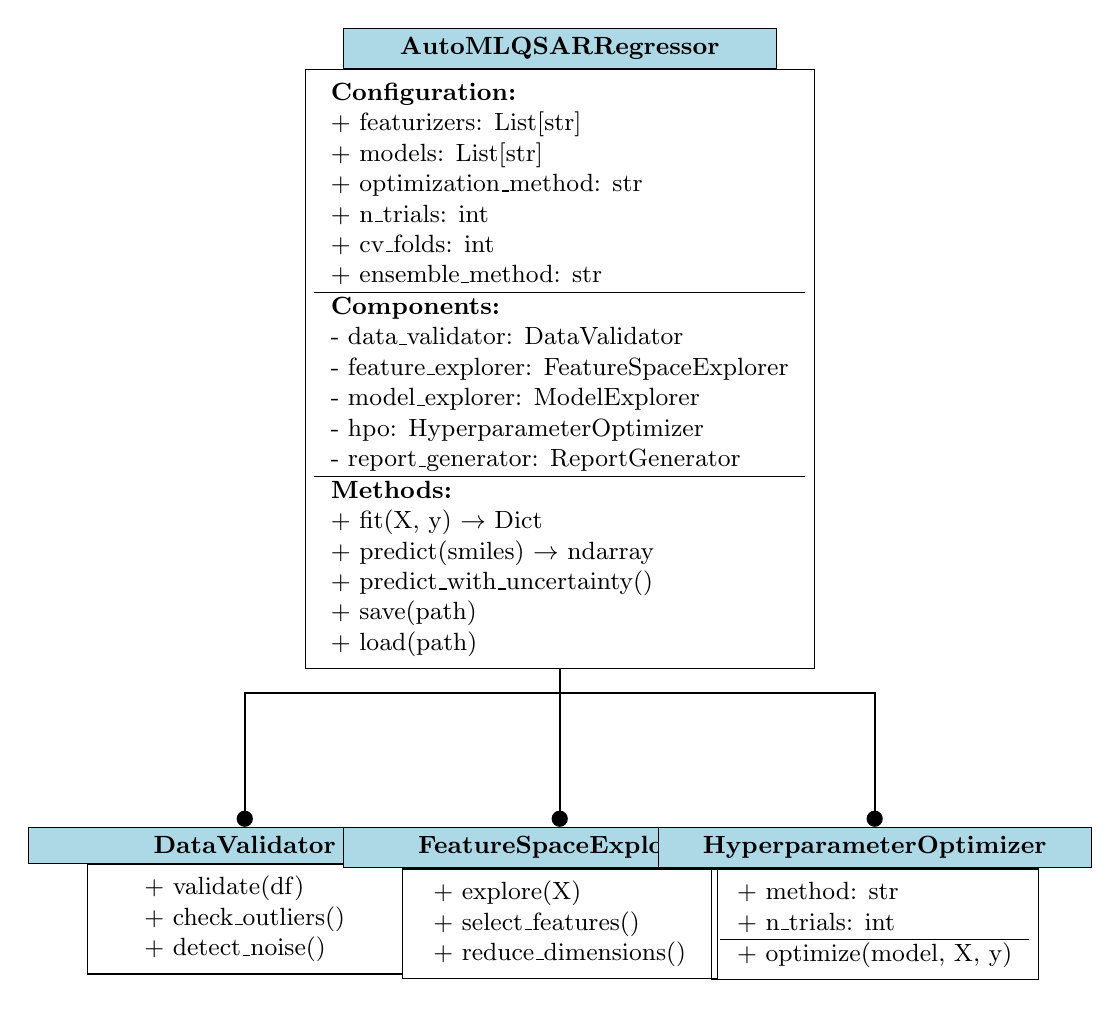
\begin{tikzpicture}[
    class/.style={rectangle, draw, minimum width=5.5cm, font=\small},
    classname/.style={rectangle, draw, fill=classcolor, minimum width=5.5cm, font=\bfseries\small},
    arrow/.style={->, >=stealth, thick},
    composition/.style={-*, thick},
    node distance=0.1cm
]

    % AutoMLQSARRegressor (Main class)
    \node[classname] (automlname) {AutoMLQSARRegressor};
    \node[class, below=0cm of automlname] (automlattr) {
        \begin{tabular}{l}
        \textbf{Configuration:}\\
        + featurizers: List[str]\\
        + models: List[str]\\
        + optimization\_method: str\\
        + n\_trials: int\\
        + cv\_folds: int\\
        + ensemble\_method: str\\
        \hline
        \textbf{Components:}\\
        - data\_validator: DataValidator\\
        - feature\_explorer: FeatureSpaceExplorer\\
        - model\_explorer: ModelExplorer\\
        - hpo: HyperparameterOptimizer\\
        - report\_generator: ReportGenerator\\
        \hline
        \textbf{Methods:}\\
        + fit(X, y) $\rightarrow$ Dict\\
        + predict(smiles) $\rightarrow$ ndarray\\
        + predict\_with\_uncertainty()\\
        + save(path)\\
        + load(path)
        \end{tabular}
    };
    
    % Component classes
    \node[classname, below=2cm of automlattr, xshift=-4cm] (validatorname) {DataValidator};
    \node[class, below=0cm of validatorname, minimum width=4cm] (validatorattr) {
        \begin{tabular}{l}
        + validate(df)\\
        + check\_outliers()\\
        + detect\_noise()
        \end{tabular}
    };
    
    \node[classname, below=2cm of automlattr] (explorername) {FeatureSpaceExplorer};
    \node[class, below=0cm of explorername, minimum width=4cm] (explorerattr) {
        \begin{tabular}{l}
        + explore(X)\\
        + select\_features()\\
        + reduce\_dimensions()
        \end{tabular}
    };
    
    \node[classname, below=2cm of automlattr, xshift=4cm] (hponame) {HyperparameterOptimizer};
    \node[class, below=0cm of hponame, minimum width=4cm] (hpoattr) {
        \begin{tabular}{l}
        + method: str\\
        + n\_trials: int\\
        \hline
        + optimize(model, X, y)
        \end{tabular}
    };
    
    % Composition relationships
    \draw[composition] (automlattr.south) -- ++(0,-0.3) -| (validatorname.north);
    \draw[composition] (automlattr.south) -- ++(0,-0.3) -- (explorername.north);
    \draw[composition] (automlattr.south) -- ++(0,-0.3) -| (hponame.north);
    
\end{tikzpicture}
\caption{AutoML Pipeline Class Diagram}
\end{figure}

% ============================================================================
\section{Sequence Diagrams}
% ============================================================================

\subsection{Training Workflow}

\begin{figure}[H]
\centering
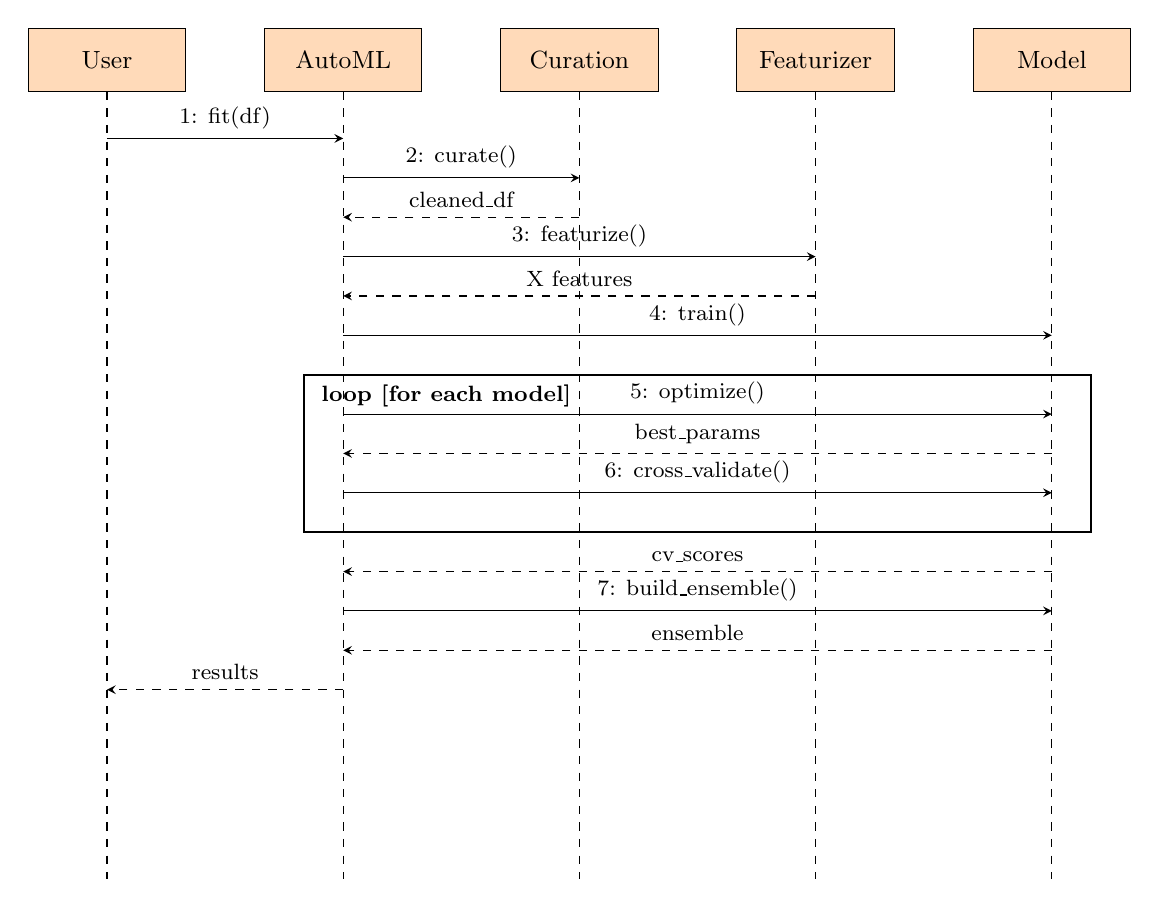
\begin{tikzpicture}[
    actor/.style={rectangle, draw, minimum width=2cm, minimum height=0.8cm, fill=interfacecolor},
    lifeline/.style={dashed},
    message/.style={->, >=stealth},
    return/.style={->, >=stealth, dashed},
    activation/.style={rectangle, draw, fill=classcolor, minimum width=0.3cm},
    font=\small
]
    % Actors
    \node[actor] (user) at (0,0) {User};
    \node[actor] (automl) at (3,0) {AutoML};
    \node[actor] (curation) at (6,0) {Curation};
    \node[actor] (feature) at (9,0) {Featurizer};
    \node[actor] (model) at (12,0) {Model};
    
    % Lifelines
    \draw[lifeline] (user.south) -- ++(0,-10);
    \draw[lifeline] (automl.south) -- ++(0,-10);
    \draw[lifeline] (curation.south) -- ++(0,-10);
    \draw[lifeline] (feature.south) -- ++(0,-10);
    \draw[lifeline] (model.south) -- ++(0,-10);
    
    % Messages
    \draw[message] (0,-1) -- node[above, font=\footnotesize] {1: fit(df)} (3,-1);
    \draw[message] (3,-1.5) -- node[above, font=\footnotesize] {2: curate()} (6,-1.5);
    \draw[return] (6,-2) -- node[above, font=\footnotesize] {cleaned\_df} (3,-2);
    
    \draw[message] (3,-2.5) -- node[above, font=\footnotesize] {3: featurize()} (9,-2.5);
    \draw[return] (9,-3) -- node[above, font=\footnotesize] {X features} (3,-3);
    
    \draw[message] (3,-3.5) -- node[above, font=\footnotesize] {4: train()} (12,-3.5);
    
    % Loop box
    \draw[thick] (2.5,-4) rectangle (12.5,-6);
    \node[anchor=north west, font=\footnotesize\bfseries] at (2.6,-4) {loop [for each model]};
    
    \draw[message] (3,-4.5) -- node[above, font=\footnotesize] {5: optimize()} (12,-4.5);
    \draw[return] (12,-5) -- node[above, font=\footnotesize] {best\_params} (3,-5);
    \draw[message] (3,-5.5) -- node[above, font=\footnotesize] {6: cross\_validate()} (12,-5.5);
    
    \draw[return] (12,-6.5) -- node[above, font=\footnotesize] {cv\_scores} (3,-6.5);
    
    \draw[message] (3,-7) -- node[above, font=\footnotesize] {7: build\_ensemble()} (12,-7);
    \draw[return] (12,-7.5) -- node[above, font=\footnotesize] {ensemble} (3,-7.5);
    
    \draw[return] (3,-8) -- node[above, font=\footnotesize] {results} (0,-8);
    
\end{tikzpicture}
\caption{Training Workflow Sequence Diagram}
\end{figure}

% ============================================================================
\section{Data Flow}
% ============================================================================

\subsection{Complete Pipeline Flow}

\begin{figure}[H]
\centering
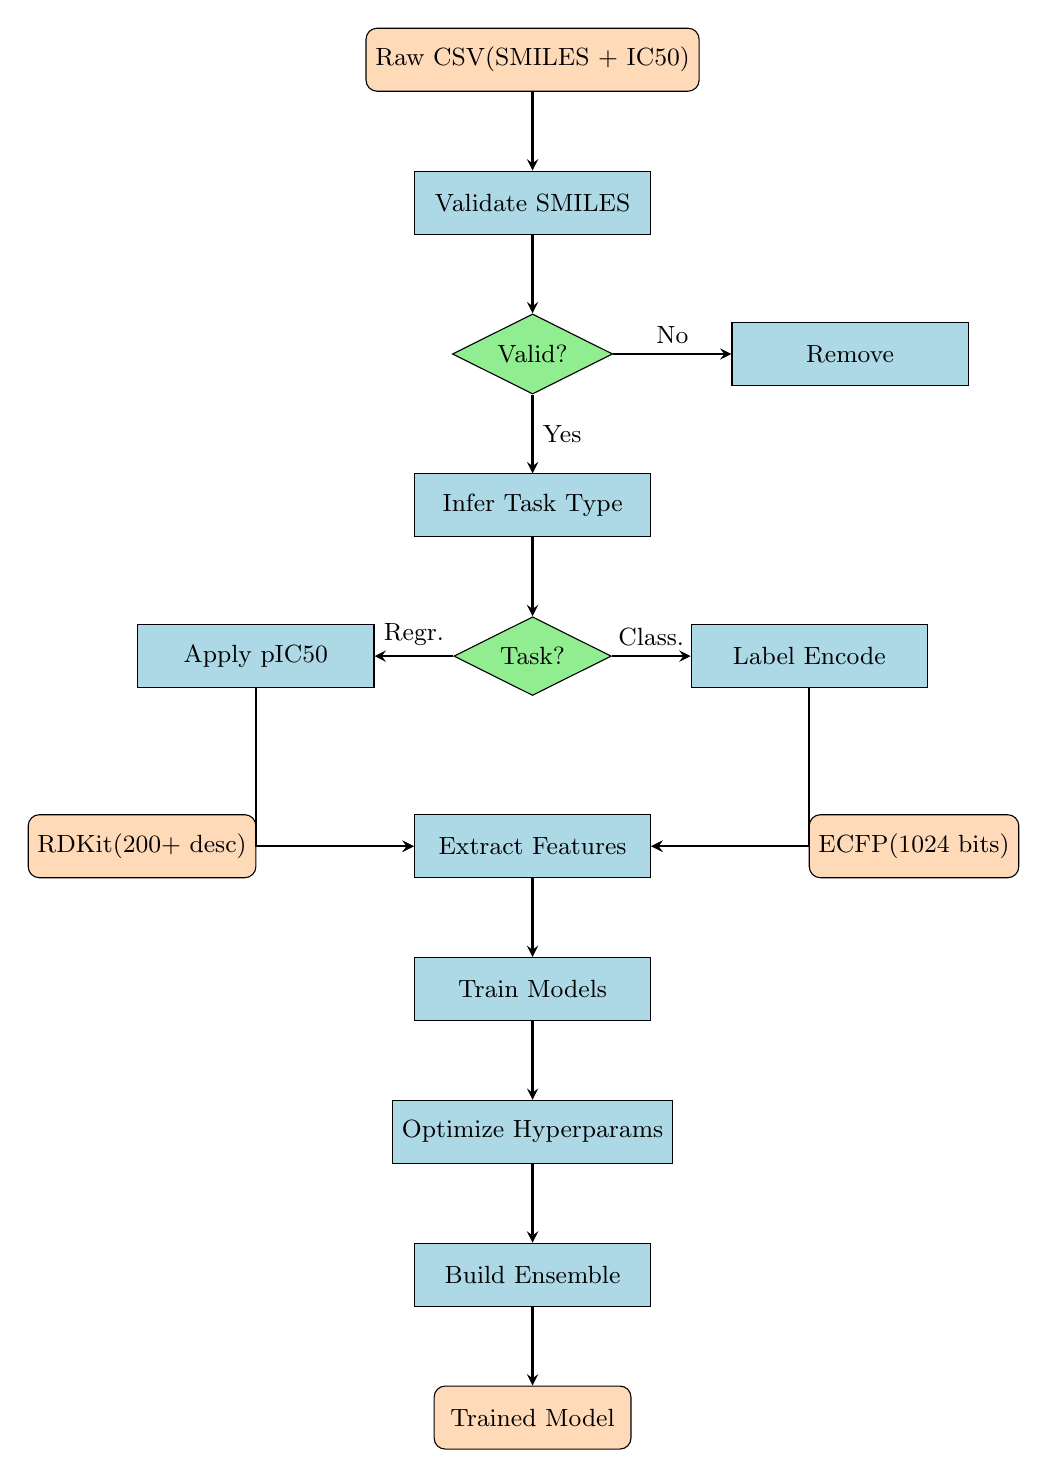
\begin{tikzpicture}[
    node distance=1cm,
    data/.style={rectangle, draw, rounded corners, minimum width=2.5cm, minimum height=0.8cm, fill=interfacecolor},
    process/.style={rectangle, draw, minimum width=3cm, minimum height=0.8cm, fill=classcolor},
    decision/.style={diamond, draw, minimum width=2cm, minimum height=1cm, fill=modulecolor, aspect=2},
    arrow/.style={->, >=stealth, thick},
    font=\small
]
    % Input
    \node[data] (input) {Raw CSV\\(SMILES + IC50)};
    
    % Curation steps
    \node[process, below=of input] (validate) {Validate SMILES};
    \node[decision, below=of validate] (valid) {Valid?};
    \node[process, right=1.5cm of valid] (remove) {Remove};
    \node[process, below=of valid] (infer) {Infer Task Type};
    
    % Task type branch
    \node[decision, below=of infer] (tasktype) {Task?};
    \node[process, left=1cm of tasktype] (regress) {Apply pIC50};
    \node[process, right=1cm of tasktype] (classify) {Label Encode};
    
    % Feature extraction
    \node[process, below=1.5cm of tasktype] (feature) {Extract Features};
    \node[data, left=2cm of feature] (rdkit) {RDKit\\(200+ desc)};
    \node[data, right=2cm of feature] (ecfp) {ECFP\\(1024 bits)};
    
    % Model training
    \node[process, below=of feature] (train) {Train Models};
    \node[process, below=of train] (optimize) {Optimize Hyperparams};
    \node[process, below=of optimize] (ensemble) {Build Ensemble};
    
    % Output
    \node[data, below=of ensemble] (output) {Trained Model};
    
    % Arrows
    \draw[arrow] (input) -- (validate);
    \draw[arrow] (validate) -- (valid);
    \draw[arrow] (valid) -- node[right] {Yes} (infer);
    \draw[arrow] (valid) -- node[above] {No} (remove);
    \draw[arrow] (infer) -- (tasktype);
    \draw[arrow] (tasktype) -- node[above] {Regr.} (regress);
    \draw[arrow] (tasktype) -- node[above] {Class.} (classify);
    \draw[arrow] (regress) |- (feature);
    \draw[arrow] (classify) |- (feature);
    \draw[arrow] (rdkit) -- (feature);
    \draw[arrow] (ecfp) -- (feature);
    \draw[arrow] (feature) -- (train);
    \draw[arrow] (train) -- (optimize);
    \draw[arrow] (optimize) -- (ensemble);
    \draw[arrow] (ensemble) -- (output);
    
\end{tikzpicture}
\caption{Complete Data Flow Diagram}
\end{figure}

% ============================================================================
\section{Supported Task Types}
% ============================================================================

\begin{table}[H]
\centering
\caption{Supported Task Types and Handling}
\begin{tabular}{@{}llll@{}}
\toprule
\textbf{Task Type} & \textbf{Example Target} & \textbf{Detection} & \textbf{Transformation} \\
\midrule
Regression (Single) & IC50\_nM & Continuous values & pIC50 (if nM/uM) \\
Regression (Multi) & IC50\_A, IC50\_B & Multiple continuous & Per-target config \\
Classification (Binary) & Active/Inactive & 2 unique strings & LabelEncoder (0/1) \\
Classification (Multiclass) & High/Medium/Low & 3+ unique strings & LabelEncoder (0,1,2...) \\
Classification (Multilabel) & [A,B], [B,C] & List values & MultiLabelBinarizer \\
Mixed & IC50 + Toxicity & Combination & Auto-detect per column \\
\bottomrule
\end{tabular}
\end{table}

% ============================================================================
\section{Model Components}
% ============================================================================

\subsection{Available Models}

The AutoML QSAR pipeline includes 12 different machine learning models spanning 5 categories.

\begin{table}[H]
\centering
\caption{Complete Model Inventory}
\begin{tabular}{@{}llp{7cm}@{}}
\toprule
\textbf{Category} & \textbf{Model} & \textbf{Description} \\
\midrule
\multirow{4}{*}{Linear} & LinearRegression & Standard OLS regression (baseline) \\
 & Ridge & L2 regularized linear regression \\
 & Lasso & L1 regularized (sparse features) \\
 & ElasticNet & L1+L2 regularization (best of both) \\
\midrule
\multirow{3}{*}{Tree-based} & RandomForest & Ensemble of decision trees with bagging \\
 & GradientBoosting & Sequential boosting (sklearn) \\
 & XGBoost & Optimized gradient boosting with regularization \\
\midrule
\multirow{2}{*}{Kernel} & SVR & Support Vector Regression (RBF kernel) \\
 & KernelRidge & Kernel Ridge Regression \\
\midrule
\multirow{2}{*}{Neural} & FeedForwardNN & MLP with configurable hidden layers \\
 & DeepNN & Deep neural network (PyTorch backend) \\
\midrule
Graph & GraphNeuralNetwork & GCN/GAT for molecular graphs \\
\bottomrule
\end{tabular}
\end{table}

\subsubsection{Model UML Class Diagram}

\begin{figure}[H]
\centering
\begin{tikzpicture}[
    class/.style={rectangle, draw, minimum width=4.5cm, font=\small},
    classname/.style={rectangle, draw, fill=classcolor, minimum width=4.5cm, font=\bfseries\small},
    abstract/.style={rectangle, draw, fill=interfacecolor, minimum width=4.5cm, font=\small},
    abstractname/.style={rectangle, draw, fill=interfacecolor!70, minimum width=4.5cm, font=\bfseries\itshape\small},
    arrow/.style={->, >=open triangle 60, thick},
    node distance=0.1cm
]

    % BaseModel (Abstract)
    \node[abstractname] (basename) {\guillemotleft abstract\guillemotright\\BaseModel};
    \node[abstract, below=0cm of basename] (baseattr) {
        \begin{tabular}{l}
        + name: str\\
        + model: sklearn.BaseEstimator\\
        \hline
        + fit(X, y) $\rightarrow$ self\\
        + predict(X) $\rightarrow$ ndarray\\
        + get\_params() $\rightarrow$ Dict
        \end{tabular}
    };
    
    % Linear models
    \node[classname, below=1.5cm of baseattr, xshift=-5cm] (ridgename) {Ridge};
    \node[class, below=0cm of ridgename, minimum width=3.5cm] (ridgeattr) {
        \begin{tabular}{l}
        + alpha: float\\
        + solver: str
        \end{tabular}
    };
    
    % Tree models
    \node[classname, below=1.5cm of baseattr, xshift=-1.5cm] (rfname) {RandomForest};
    \node[class, below=0cm of rfname, minimum width=3.5cm] (rfattr) {
        \begin{tabular}{l}
        + n\_estimators: int\\
        + max\_depth: int\\
        + min\_samples\_split: int
        \end{tabular}
    };
    
    % XGBoost
    \node[classname, below=1.5cm of baseattr, xshift=2cm] (xgbname) {XGBoost};
    \node[class, below=0cm of xgbname, minimum width=3.5cm] (xgbattr) {
        \begin{tabular}{l}
        + n\_estimators: int\\
        + learning\_rate: float\\
        + max\_depth: int\\
        + reg\_alpha: float\\
        + reg\_lambda: float
        \end{tabular}
    };
    
    % Neural models
    \node[classname, below=1.5cm of baseattr, xshift=5.5cm] (nnname) {FeedForwardNN};
    \node[class, below=0cm of nnname, minimum width=3.5cm] (nnattr) {
        \begin{tabular}{l}
        + hidden\_layers: List[int]\\
        + activation: str\\
        + learning\_rate: float\\
        + max\_iter: int
        \end{tabular}
    };
    
    % Inheritance arrows
    \draw[arrow] (ridgename.north) -- ++(0,0.4) -| (baseattr.south);
    \draw[arrow] (rfname.north) -- ++(0,0.4) -| (baseattr.south);
    \draw[arrow] (xgbname.north) -- ++(0,0.4) -| (baseattr.south);
    \draw[arrow] (nnname.north) -- ++(0,0.4) -| (baseattr.south);
    
\end{tikzpicture}
\caption{Model Hierarchy Class Diagram}
\end{figure}

\subsubsection{Neural Network Architecture}

\begin{table}[H]
\centering
\caption{Neural Network Model Configurations}
\begin{tabular}{@{}llp{6cm}@{}}
\toprule
\textbf{Model} & \textbf{Architecture} & \textbf{Hyperparameters} \\
\midrule
FeedForwardNN & Input $\rightarrow$ [100, 50] $\rightarrow$ Output & 
\begin{tabular}[t]{@{}l@{}}
hidden\_layers: [100, 50]\\
activation: relu, tanh, sigmoid\\
learning\_rate: 0.001\\
max\_iter: 200\\
early\_stopping: True
\end{tabular} \\
\midrule
DeepNN & Input $\rightarrow$ [256, 128, 64] $\rightarrow$ Output & 
\begin{tabular}[t]{@{}l@{}}
hidden\_layers: [256, 128, 64]\\
dropout: 0.2\\
learning\_rate: 0.001\\
epochs: 100\\
batch\_size: 32\\
GPU support: Auto-detect
\end{tabular} \\
\midrule
GraphNeuralNetwork & Atoms $\rightarrow$ GCN Layers $\rightarrow$ Pool $\rightarrow$ Output & 
\begin{tabular}[t]{@{}l@{}}
hidden\_channels: 64\\
num\_layers: 3\\
dropout: 0.2\\
pooling: global\_mean\_pool
\end{tabular} \\
\bottomrule
\end{tabular}
\end{table}

\subsubsection{Model Hyperparameter Spaces}

\begin{table}[H]
\centering
\caption{Hyperparameter Search Spaces for Bayesian Optimization}
\begin{tabular}{@{}llll@{}}
\toprule
\textbf{Model} & \textbf{Parameter} & \textbf{Type} & \textbf{Range} \\
\midrule
\multirow{2}{*}{Ridge} & alpha & log-uniform & [1e-4, 1e2] \\
 & solver & categorical & [auto, svd, cholesky] \\
\midrule
\multirow{3}{*}{RandomForest} & n\_estimators & int & [50, 500] \\
 & max\_depth & int & [3, 20] \\
 & min\_samples\_split & int & [2, 20] \\
\midrule
\multirow{4}{*}{XGBoost} & n\_estimators & int & [50, 500] \\
 & learning\_rate & log-uniform & [0.01, 0.3] \\
 & max\_depth & int & [3, 12] \\
 & reg\_lambda & log-uniform & [1e-3, 10] \\
\midrule
\multirow{3}{*}{SVR} & C & log-uniform & [0.1, 100] \\
 & epsilon & uniform & [0.01, 0.5] \\
 & gamma & categorical & [scale, auto] \\
\bottomrule
\end{tabular}
\end{table}

\subsection{Featurization Methods}

The pipeline supports 7 distinct molecular featurization methods across 4 categories.

\begin{table}[H]
\centering
\caption{Complete Featurization Inventory}
\begin{tabular}{@{}lclp{5.5cm}@{}}
\toprule
\textbf{Method} & \textbf{Dims} & \textbf{Type} & \textbf{Description} \\
\midrule
RDKit Descriptors & 200+ & Float & Physicochemical properties \\
ECFP Fingerprints & 1024 & Binary & Circular substructures (Morgan) \\
MACCS Keys & 167 & Binary & MDL public structure keys \\
Pharmacophore & 28+ & Float & H-bond donors/acceptors, aromatics \\
Mol2Vec Embeddings & 300 & Float & Pre-trained molecular vectors \\
Graph Features & 44+6 & Mixed & Node \& edge features for GNN \\
Random Embeddings & 128 & Float & Placeholder for custom models \\
\bottomrule
\end{tabular}
\end{table}

\subsubsection{Featurization UML Class Diagram}

\begin{figure}[H]
\centering
\begin{tikzpicture}[
    class/.style={rectangle, draw, minimum width=4cm, font=\small},
    classname/.style={rectangle, draw, fill=classcolor, minimum width=4cm, font=\bfseries\small},
    abstract/.style={rectangle, draw, fill=interfacecolor, minimum width=5cm, font=\small},
    abstractname/.style={rectangle, draw, fill=interfacecolor!70, minimum width=5cm, font=\bfseries\itshape\small},
    arrow/.style={->, >=open triangle 60, thick},
    node distance=0.1cm
]

    % BaseFeaturizer (Abstract)
    \node[abstractname] (basename) {\guillemotleft abstract\guillemotright\\BaseFeaturizer};
    \node[abstract, below=0cm of basename] (baseattr) {
        \begin{tabular}{l}
        + name: str\\
        + feature\_names: List[str]\\
        \hline
        + featurize(molecules) $\rightarrow$ ndarray\\
        \# \_smiles\_to\_mol(smiles) $\rightarrow$ Mol\\
        \# \_prepare\_molecules(mols) $\rightarrow$ List
        \end{tabular}
    };
    
    % Row 1: Traditional descriptors
    \node[classname, below=1.8cm of baseattr, xshift=-5cm] (rdkitname) {RDKitDescriptors};
    \node[class, below=0cm of rdkitname] (rdkitattr) {
        \begin{tabular}{l}
        + descriptors: 200+\\
        + includes: LogP, MW,\\
        \hspace{2mm}TPSA, HBA, HBD
        \end{tabular}
    };
    
    \node[classname, below=1.8cm of baseattr, xshift=-1cm] (ecfpname) {ECFPFingerprints};
    \node[class, below=0cm of ecfpname] (ecfpattr) {
        \begin{tabular}{l}
        + radius: 2 (ECFP4)\\
        + n\_bits: 1024\\
        + use\_features: bool
        \end{tabular}
    };
    
    \node[classname, below=1.8cm of baseattr, xshift=3cm] (maccsname) {MACCSFingerprints};
    \node[class, below=0cm of maccsname] (maccsattr) {
        \begin{tabular}{l}
        + n\_bits: 167\\
        + predefined keys
        \end{tabular}
    };
    
    % Row 2: Advanced features
    \node[classname, below=3.8cm of baseattr, xshift=-5cm] (pharmname) {PharmacophoreFeatures};
    \node[class, below=0cm of pharmname] (pharmattr) {
        \begin{tabular}{l}
        + Donor, Acceptor\\
        + PosIonizable, NegIonizable\\
        + Aromatic, Hydrophobe
        \end{tabular}
    };
    
    \node[classname, below=3.8cm of baseattr, xshift=-0.5cm] (graphname) {GraphFeaturizer};
    \node[class, below=0cm of graphname] (graphattr) {
        \begin{tabular}{l}
        + atom\_features: 44\\
        + bond\_features: 6\\
        + edge\_index: COO
        \end{tabular}
    };
    
    \node[classname, below=3.8cm of baseattr, xshift=3.5cm] (embname) {MolecularEmbeddings};
    \node[class, below=0cm of embname] (embattr) {
        \begin{tabular}{l}
        + embedding\_type: str\\
        + embedding\_dim: 128\\
        + mol2vec: 300
        \end{tabular}
    };
    
    % Inheritance arrows
    \draw[arrow] (rdkitname.north) -- ++(0,0.5) -| (baseattr.south);
    \draw[arrow] (ecfpname.north) -- ++(0,0.5) -| (baseattr.south);
    \draw[arrow] (maccsname.north) -- ++(0,0.5) -| (baseattr.south);
    \draw[arrow] (pharmname.north) -- ++(0,0.3) -| ([xshift=-1cm]baseattr.south);
    \draw[arrow] (graphname.north) -- ++(0,0.3) -- ++(0,0.2) -| (baseattr.south);
    \draw[arrow] (embname.north) -- ++(0,0.3) -| ([xshift=1cm]baseattr.south);
    
\end{tikzpicture}
\caption{Complete Featurization Module Class Diagram}
\end{figure}

\subsubsection{RDKit Molecular Descriptors}

\begin{table}[H]
\centering
\caption{Key RDKit Molecular Descriptors}
\begin{tabular}{@{}lll@{}}
\toprule
\textbf{Category} & \textbf{Descriptors} & \textbf{Description} \\
\midrule
Physical & MolWt, HeavyAtomMolWt & Molecular weight \\
 & ExactMolWt & Exact molecular weight \\
\midrule
Lipophilicity & MolLogP, TPSA & Partition coefficient, polar surface area \\
\midrule
H-bonding & NumHDonors, NumHAcceptors & Hydrogen bond donors/acceptors \\
 & NHOHCount, NOCount & N-H/O-H count, N/O count \\
\midrule
Structural & NumRotatableBonds & Rotatable bond count \\
 & NumAromaticRings & Aromatic ring count \\
 & FractionCSP3 & Fraction of sp3 carbons \\
\midrule
Topological & BalabanJ, BertzCT & Graph complexity indices \\
 & Chi0, Chi1, Kappa1 & Connectivity indices \\
\midrule
Electronic & MaxPartialCharge & Maximum partial charge \\
 & MinPartialCharge & Minimum partial charge \\
\bottomrule
\end{tabular}
\end{table}

\subsubsection{Fingerprint Comparison}

\begin{table}[H]
\centering
\caption{Molecular Fingerprint Comparison}
\begin{tabular}{@{}llll@{}}
\toprule
\textbf{Fingerprint} & \textbf{ECFP} & \textbf{MACCS} & \textbf{Use Case} \\
\midrule
Encoding & Circular & Predefined & - \\
Bits & 1024 (configurable) & 167 (fixed) & - \\
Radius & 2 (ECFP4), 3 (ECFP6) & N/A & - \\
Substructures & Learned & Expert-defined & - \\
Speed & Fast & Very fast & - \\
Best for & Similarity, ML & Substructure search & - \\
\bottomrule
\end{tabular}
\end{table}

\subsubsection{Pharmacophore Feature Types}

\begin{table}[H]
\centering
\caption{Pharmacophore Feature Definitions}
\begin{tabular}{@{}llp{6cm}@{}}
\toprule
\textbf{Feature Type} & \textbf{Symbol} & \textbf{Description} \\
\midrule
Hydrogen Bond Donor & HBD & Atoms that donate H in H-bonds (e.g., -NH, -OH) \\
Hydrogen Bond Acceptor & HBA & Atoms that accept H in H-bonds (e.g., C=O, -N<) \\
Positive Ionizable & PI & Groups that can be positively charged at physiological pH \\
Negative Ionizable & NI & Groups that can be negatively charged at physiological pH \\
Aromatic & Ar & Aromatic ring systems \\
Hydrophobe & Hy & Hydrophobic regions (alkyl, aromatic) \\
Lumped Hydrophobe & LH & Extended hydrophobic regions \\
\bottomrule
\end{tabular}
\end{table}

\subsubsection{Graph Features for GNN}

The GraphFeaturizer converts molecules into graph representations suitable for Graph Neural Networks.

\begin{table}[H]
\centering
\caption{Atom (Node) Feature Vector (44 dimensions)}
\begin{tabular}{@{}lll@{}}
\toprule
\textbf{Feature} & \textbf{Encoding} & \textbf{Dimensions} \\
\midrule
Atom Type & One-hot [C, N, O, S, F, Si, P, Cl, Br, I, Other] & 11 \\
Degree & One-hot [0, 1, 2, 3, 4, 5, 5+] & 7 \\
Formal Charge & One-hot [-2, -1, 0, +1, +2] & 5 \\
Hybridization & One-hot [SP, SP2, SP3, SP3D, SP3D2, Other] & 6 \\
Is Aromatic & Binary & 1 \\
Num Radical Electrons & Integer & 1 \\
Total Num H & Integer & 1 \\
Is In Ring & Binary & 1 \\
\midrule
\textbf{Total} & & \textbf{44} \\
\bottomrule
\end{tabular}
\end{table}

\begin{table}[H]
\centering
\caption{Bond (Edge) Feature Vector (6 dimensions)}
\begin{tabular}{@{}lll@{}}
\toprule
\textbf{Feature} & \textbf{Encoding} & \textbf{Dimensions} \\
\midrule
Bond Type & One-hot [Single, Double, Triple, Aromatic] & 4 \\
Is Conjugated & Binary & 1 \\
Is In Ring & Binary & 1 \\
\midrule
\textbf{Total} & & \textbf{6} \\
\bottomrule
\end{tabular}
\end{table}

\subsection{Ensemble Methods}

The pipeline supports multiple ensemble strategies for combining predictions from multiple models.

\begin{table}[H]
\centering
\caption{Available Ensemble Methods}
\begin{tabular}{@{}llp{6.5cm}@{}}
\toprule
\textbf{Method} & \textbf{Class} & \textbf{Description} \\
\midrule
Voting & VotingEnsemble & Average predictions from all models (weighted or unweighted) \\
Stacking & StackingEnsemble & Meta-learner trained on base model predictions \\
Top-K & TopKEnsemble & Select K best models based on CV performance \\
\bottomrule
\end{tabular}
\end{table}

\subsubsection{Ensemble UML Class Diagram}

\begin{figure}[H]
\centering
\begin{tikzpicture}[
    class/.style={rectangle, draw, minimum width=4.5cm, font=\small},
    classname/.style={rectangle, draw, fill=classcolor, minimum width=4.5cm, font=\bfseries\small},
    abstract/.style={rectangle, draw, fill=interfacecolor, minimum width=5cm, font=\small},
    abstractname/.style={rectangle, draw, fill=interfacecolor!70, minimum width=5cm, font=\bfseries\itshape\small},
    arrow/.style={->, >=open triangle 60, thick},
    node distance=0.1cm
]

    % BaseEnsemble (Abstract)
    \node[abstractname] (basename) {\guillemotleft abstract\guillemotright\\BaseEnsemble};
    \node[abstract, below=0cm of basename] (baseattr) {
        \begin{tabular}{l}
        + models: List[BaseModel]\\
        + weights: List[float]\\
        \hline
        + fit(X, y) $\rightarrow$ self\\
        + predict(X) $\rightarrow$ ndarray\\
        \# \_combine\_predictions()
        \end{tabular}
    };
    
    % Voting
    \node[classname, below=1.8cm of baseattr, xshift=-4cm] (votename) {VotingEnsemble};
    \node[class, below=0cm of votename] (voteattr) {
        \begin{tabular}{l}
        + voting: str\\
        \hspace{2mm}(mean, median)\\
        + weighted: bool
        \end{tabular}
    };
    
    % Stacking
    \node[classname, below=1.8cm of baseattr] (stackname) {StackingEnsemble};
    \node[class, below=0cm of stackname] (stackattr) {
        \begin{tabular}{l}
        + meta\_learner: BaseModel\\
        + cv\_folds: int\\
        + passthrough: bool
        \end{tabular}
    };
    
    % Top-K
    \node[classname, below=1.8cm of baseattr, xshift=4cm] (topkname) {TopKEnsemble};
    \node[class, below=0cm of topkname] (topkattr) {
        \begin{tabular}{l}
        + k: int\\
        + metric: str\\
        + cv\_scores: Dict
        \end{tabular}
    };
    
    % Inheritance arrows
    \draw[arrow] (votename.north) -- ++(0,0.5) -| (baseattr.south);
    \draw[arrow] (stackname.north) -- (baseattr.south);
    \draw[arrow] (topkname.north) -- ++(0,0.5) -| (baseattr.south);
    
\end{tikzpicture}
\caption{Ensemble Methods Class Diagram}
\end{figure}

\subsubsection{Ensemble Strategy Comparison}

\begin{table}[H]
\centering
\caption{Ensemble Strategy Comparison}
\begin{tabular}{@{}llll@{}}
\toprule
\textbf{Strategy} & \textbf{Pros} & \textbf{Cons} & \textbf{Best For} \\
\midrule
Voting & Simple, fast, robust & Equal treatment & Diverse models \\
Stacking & Learns optimal combination & Risk of overfitting & Large datasets \\
Top-K & Focus on best performers & Ignores diversity & Limited compute \\
\bottomrule
\end{tabular}
\end{table}

\subsection{Optimization Methods}

\begin{table}[H]
\centering
\caption{Hyperparameter Optimization Methods}
\begin{tabular}{@{}llp{6cm}@{}}
\toprule
\textbf{Method} & \textbf{Class} & \textbf{Description} \\
\midrule
Bayesian & BayesianOptimization & TPE sampler with Optuna, efficient search \\
Grid Search & GridSearchCV & Exhaustive search over parameter grid \\
Genetic & GeneticOptimization & Evolutionary algorithm for global optimization \\
\bottomrule
\end{tabular}
\end{table}

% ============================================================================
\section{API Reference}
% ============================================================================

\subsection{QSARDataCurationAgent}

\begin{lstlisting}[caption={Data Curation Usage}]
from automl_qsar.preprocessing import QSARDataCurationAgent

# Initialize with DataFrame
agent = QSARDataCurationAgent(
    df=dataframe,           # pandas DataFrame
    smiles_col='SMILES',    # SMILES column name
    target_cols='IC50_nM',  # Target column(s)
    units='nM',             # Units for pIC50 transform
    verbose=True            # Print progress
)

# Run curation
cleaned_df = agent.run()

# Get statistics
stats = agent.get_statistics()
# Returns: {'overall_task': 'regression_single', 
#           'n_original': 100, 'n_cleaned': 95, ...}

# Get target configurations
configs = agent.get_target_configs()
# Returns: {'IC50_nM': TargetConfig(...)}

# Get label encoder (for classification)
encoder = agent.get_label_encoder('Activity')
original_labels = encoder.inverse_transform([0, 1])
\end{lstlisting}

\subsection{AutoMLQSARRegressor}

\begin{lstlisting}[caption={AutoML Pipeline Usage}]
from automl_qsar import AutoMLQSAR

# Initialize
automl = AutoMLQSAR(
    featurizers=['rdkit', 'ecfp'],  # Feature types
    models=['ridge', 'randomforest', 'xgboost'],
    optimization_method='bayesian',
    n_trials=50,           # Optimization trials
    cv_folds=5,            # Cross-validation folds
    ensemble_method='topk', # Ensemble strategy
    random_state=42
)

# Train
results = automl.fit(X, y)

# Predict
predictions = automl.predict(new_smiles)

# Predict with uncertainty
pred, uncertainty = automl.predict_with_uncertainty(smiles)

# Save/Load
automl.save('./model_path')
automl.load('./model_path')
\end{lstlisting}

% ============================================================================
\section{Metrics and Evaluation}
% ============================================================================

\subsection{Regression Metrics}

\begin{align}
\text{RMSE} &= \sqrt{\frac{1}{n}\sum_{i=1}^{n}(y_i - \hat{y}_i)^2} \\[0.5em]
\text{MAE} &= \frac{1}{n}\sum_{i=1}^{n}|y_i - \hat{y}_i| \\[0.5em]
R^2 &= 1 - \frac{\sum_{i=1}^{n}(y_i - \hat{y}_i)^2}{\sum_{i=1}^{n}(y_i - \bar{y})^2}
\end{align}

\subsection{Activity Classification}

\begin{table}[H]
\centering
\caption{IC50 Activity Classification}
\begin{tabular}{@{}ccc@{}}
\toprule
\textbf{IC50 Range} & \textbf{pIC50 Range} & \textbf{Activity Class} \\
\midrule
$<$ 100 nM & $>$ 7.0 & Strong (Potent) \\
100--1000 nM & 6.0--7.0 & Moderate \\
$>$ 1000 nM & $<$ 6.0 & Weak/Inactive \\
\bottomrule
\end{tabular}
\end{table}

% ============================================================================
\section{Testing and CI/CD}
% ============================================================================

\subsection{Test Structure}

\begin{verbatim}
tests/
├── conftest.py              # Shared fixtures
├── unit/                    # Unit tests (29 tests)
│   ├── test_data_curation.py
│   ├── test_featurizers.py
│   └── test_models.py
├── integration/             # Integration tests (7 tests)
│   └── test_full_pipeline.py
└── scenarios/               # Scenario tests (27 tests)
    ├── test_regression_single.py
    ├── test_regression_multi.py
    ├── test_classification_binary.py
    ├── test_classification_multiclass.py
    ├── test_mixed_tasks.py
    └── test_large_dataset.py
\end{verbatim}

\subsection{CI/CD Pipeline}

The GitHub Actions workflow runs on every push:

\begin{enumerate}
    \item \textbf{Lint}: Code style check with flake8
    \item \textbf{Unit Tests}: Python 3.9, 3.10, 3.11 matrix
    \item \textbf{Integration Tests}: Full pipeline validation
    \item \textbf{Scenario Tests}: Real-world use cases
    \item \textbf{Coverage}: Code coverage reporting
\end{enumerate}

% ============================================================================
\section{Conclusion}
% ============================================================================

The AutoML QSAR Pipeline provides a comprehensive, automated solution for molecular activity prediction. Key strengths include:

\begin{itemize}
    \item \textbf{Automation}: Minimal manual intervention required
    \item \textbf{Flexibility}: Supports multiple task types and configurations
    \item \textbf{Robustness}: Extensive validation and error handling
    \item \textbf{Reproducibility}: Fixed random states and comprehensive logging
    \item \textbf{Extensibility}: Modular design allows easy addition of new methods
\end{itemize}

For questions or contributions, please refer to the project repository.

\end{document}
